\chapter{Instahub}

\section{Aufgabe 1: Einrichtung des sozialen Netzwerks}
\label{sec:aufg1}
% credits to Rainer Winkler for this tutorial
\begin{table}[H]
\centering
\begin{tabular}{r|l}
 \emoji{chequered-flag} & Selber eine Datenbank administrieren \\\hline
 \emoji{family-man-woman-girl-boy} & 3er- bis 4er-Gruppen \\\hline
 \emoji{stopwatch} & ca. 25 min.
\end{tabular}
\end{table}

Führen Sie folgende Schritte aus:
 
\begin{enumerate}
	\item Bestimmen Sie jemanden als \textcolor{RoyalBlue}{AdministratorIn}. Die anderen Personen sind  \textcolor{ForestGreen}{BenutzerInnen}. Die unten stehenden \textcolor{RoyalBlue}{Administratoren}-Schritte sollten von \textbf{allen} ausgeführt werden, damit jeder sein eigenes soziales Netzwerk erstellt, da dieses später verwendet wird.
	\item \textcolor{RoyalBlue}{AdministratorIn}: Auf \url{https://instahub.org} gehen 
	\item \textcolor{RoyalBlue}{AdministratorIn}: Auf Hub erstellen (rechts oben) klicken und einen Hub erstellen. 
	\begin{figure}[H]
	\centering
	
\includegraphics[width=1.5cm]{GrundlagenInfo/DataScience/06_Daten/Figures/tutorial-instahub-1}
	\end{figure}
	\item \textcolor{RoyalBlue}{AdministratorIn}: Geben Sie folgende Angaben ein:
	\begin{itemize}
		\item Lehrername: \texttt{cyrilwendl}.
		\item Username ist \texttt{admin} und kann nicht geändert werden.
		\item Ihren Namen und Ihr Passwort können Sie frei setzen. Das Passwort sollten Sie sich irgendwo notieren.
		\item Sie können entweder eine echte Email-Adresse angeben oder die generierte Emailadresse so lassen. Dann können Sie jedoch ihr Passwort nicht mehr per Mail zurücksetzen, falls Sie dieses je verlieren sollten.
	\end{itemize} Ich muss nun Ihren Hub (=ihre Webseite) manuell aktivieren. Dies sollte innerhalb weniger Sekunden geschehen sein.
	\begin{figure}[H]
	\centering
	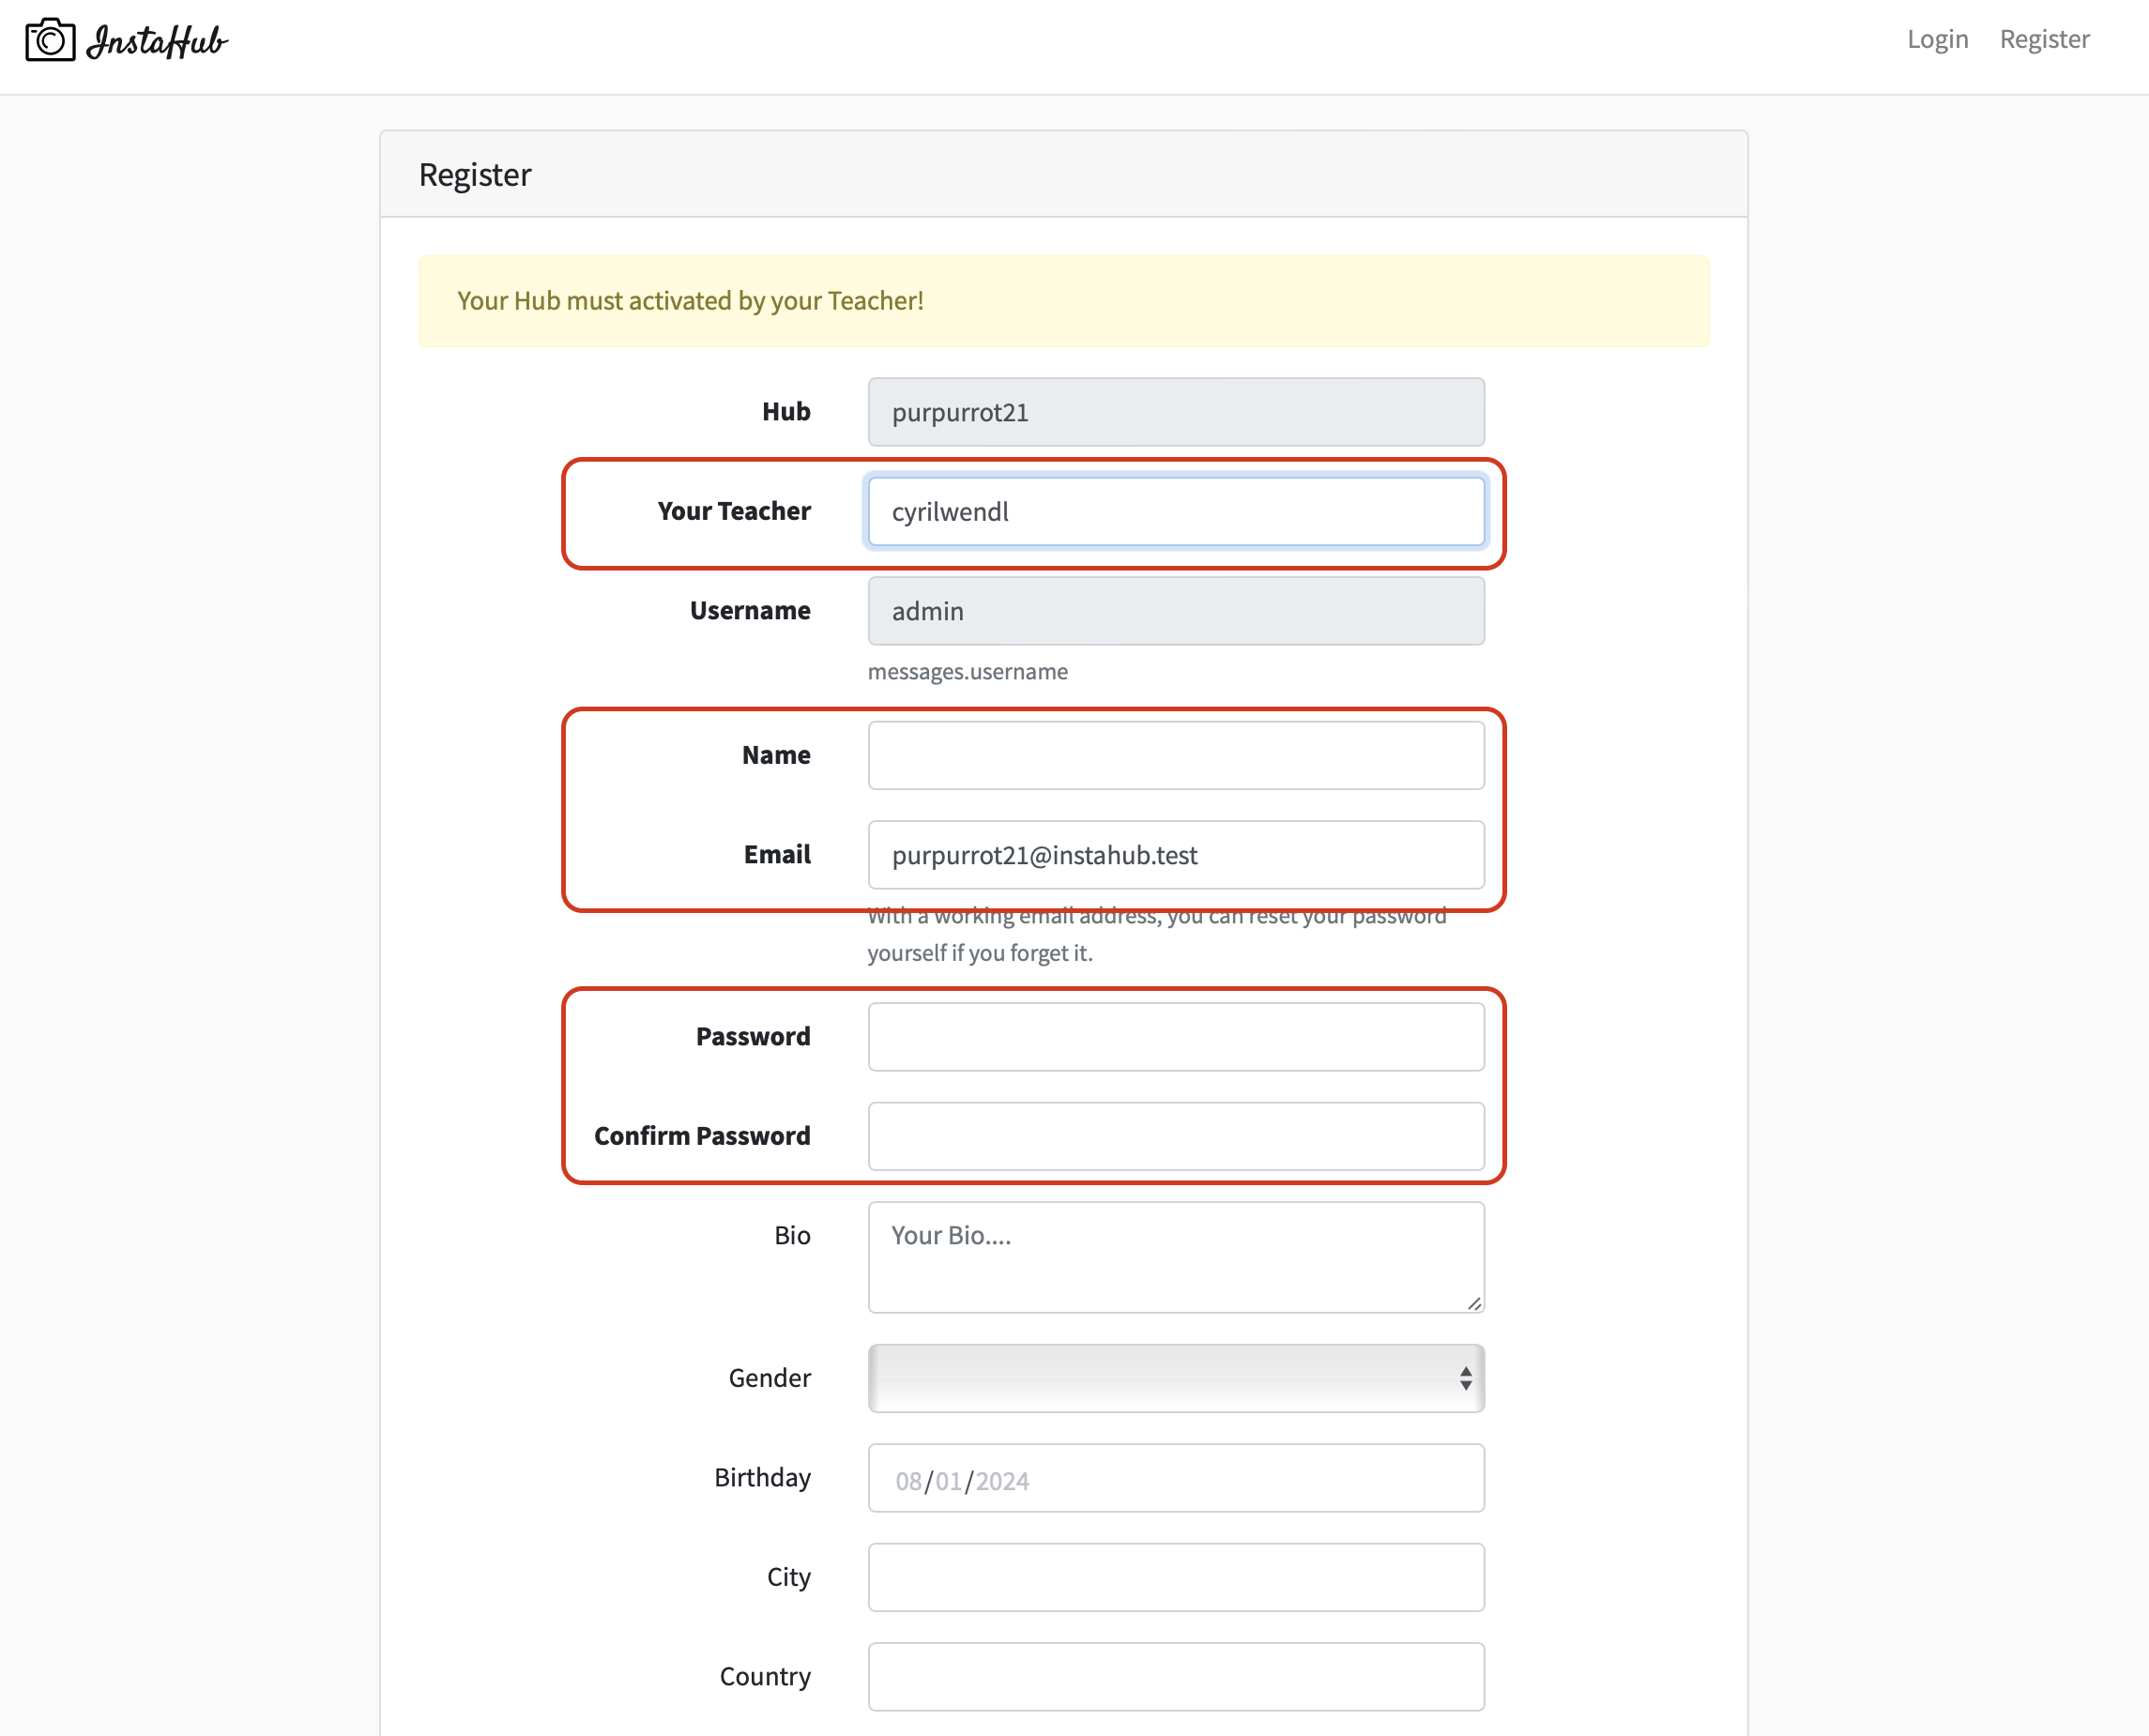
\includegraphics[width=.5\textwidth]{GrundlagenInfo/DataScience/06_Daten/Figures/tutorial-instahub-2}
	\end{figure}	
	\item Sobald ich als Lehrperson die Accounts aktiviert habe, können Ihre Kollegen das soziale Netzwerk betreten, indem sie folgende URL eingeben: \url{https://namedesnetzwerks.instahub.org} (im Beispiel oben wäre das \url{https://purpurrot21.instahub.org}) und können dort einen Account erstellen, bzw. sich anmelden.
	\begin{itemize}
		\item \textcolor{RoyalBlue}{AdministratorIn}: Mit Benutzername \texttt{admin} und dem von Ihnen zuvor gewählten Passwort anmelden. Sie sind nun AdministratorIn Ihres eigenen sozialen Netzwerks.
		\item \textcolor{ForestGreen}{BenutzerInnen}: Gehen Sie auf die von der Administratorin erstellte Webseite (\url{https://namedesnetzwerks.instahub.org}, wobei ``\texttt{namedesnetzwerks}'' ersetzt werden muss) und erstellen Sie ein neues Konto für sich.
	\end{itemize}
	\item \textcolor{RoyalBlue}{AdministratorIn}: Die neuen Accounts der \textcolor{ForestGreen}{BenutzerInnen} muss dann von Ihnen als \textcolor{RoyalBlue}{AdministratorIn} aktiviert werden, indem Sie den User suchen, auf ``Bearbeiten'' und dann ganz unten auf ``Account ist freigeschaltet'' klicken.  
	\item \textcolor{RoyalBlue}{AdministratorIn} und \textcolor{ForestGreen}{BenutzerIn}: Posten Sie nun falls Sie möchten Bilder in den sozialen Netzwerken Ihrer Kollegen, vergeben Sie Likes, folgen Sie anderen und kommentieren Sie fleissig in den anderen Netzwerken (max. 5 Minuten).
\end{enumerate}

\section{Aufgabe 2: SQL-Abfragen}

\begin{table}[H]
\centering
\begin{tabular}{r|l}
 \emoji{chequered-flag} & Lernen, mithilfe von SQL eigene Abfragen zu machen \\\hline
 \emoji{stopwatch} & ca. 60 min.
\end{tabular}
\end{table}
 
Öffnen Sie folgenden Link: \url{https://wi-wissen.github.io/instahub-doc-de/#/exercices}. 

Lösen Sie folgende Abschnitte mithilfe Ihrer eigenen InstaHub-Webseite, die Sie in Aufgabe \ref{sec:aufg1} erstellt haben.
\begin{itemize}
\item ``Auswerten von Daten I''
\item ``Verändern von Daten I''
\end{itemize} 
